\caulc
\Opensolutionfile{ans}[ans/ansTN-Dung]
%%%=============EX_1=============%%%
\begin{ex}%[Nguyễn Văn Sang]%[TDMT05]%[1D1N5-3]
	Nghiệm của phương trình $8\cos\left(x - \dfrac{\pi}{4}\right) = 8$ là
	\choice
	{$x \in \varnothing$}
	{$x = \dfrac{\pi}{4} + k\pi, k \in \mathbb{Z}$}
	{$x = \dfrac{\pi}{4} + k2\pi, k \in \mathbb{N}$}
	{\True $x = \dfrac{\pi}{4} + k2\pi, k \in \mathbb{Z}$}
	\loigiai{
		Ta có
		\begin{eqnarray*}
			& & 8\cos\left(x - \dfrac{\pi}{4}\right) = 8\\
			& \Leftrightarrow & \cos\left(x - \dfrac{\pi}{4}\right) = 1 \\
			& \Leftrightarrow & x - \dfrac{\pi}{4} = k2\pi \\
			& \Leftrightarrow & x = \dfrac{\pi}{4} + k2\pi, \, (k \in \mathbb{Z}).
		\end{eqnarray*}
	}
\end{ex}
%%%=============================%%%

%%%=============EX_2=============%%%
\begin{ex}%[2D1N3-2]
	Cho bảng biến thiên của hàm số $y=f(x)$ như hình vẽ bên dưới. Giá trị nhỏ nhất của hàm số $y=f(x)$ trên khoảng $(0;+\infty)$ bằng
	\begin{center}
		\begin{tikzpicture}[font=\normalsize,t style/.style={style=solid}]
			\tkzTabInit[nocadre=false, lgt=1.2, espcl=2.5, deltacl=0.5]
			{$x$/0.6,$f(x)$/2}
			{$-\infty$, $-2$, $0$, $4$, $+\infty$}
			
			\path
			($(N12)!0.8!(N11)$) node (A1){$+\infty$}
			($(N22)!0.1!(N21)$) node (A2){$-5 $}
			($(N32)!0.8!(N31)$) node (A3){$ 12 $}
			($(N42)!0.3!(N41)$) node (A4){$ 3$}
			($(N52)!0.8!(N51)$) node (A5){$ +\infty$};
			
			\foreach \x/\y in {A1/A2, A2/A3, A3/A4, A4/A5}{
				\draw[-stealth] (\x)--(\y);
			}
		\end{tikzpicture}
	\end{center}
	\choice
	{\True $3$}
	{$-5$}
	{$-2$}
	{$4$}
	\loigiai{
		Theo bảng biến thiên, ta có $\min\limits_{(0;+\infty)}f(x)=3$
	}
\end{ex}
%%%=============================%%%

%%%=============EX_3=============%%%
\begin{ex}%[1D6N4-4]%[TDMT05]%[Nguyễn Trí Minh Tuấn]
	Nghiệm của phương trình $4^{x^2-2}=128$ là
	\choice
	{\True $\left\{\pm\dfrac{\sqrt{22}}{2}\right\}$}
	{$\left\{\pm 2\right\}$}
	{$\left\{\pm 3\right\}$}
	{$\left\{3\right\}$}
	\loigiai{
		Do $4=2^2$ và $128=2^7$ nên
		\[
		4^{x^2-2}=128 \Leftrightarrow 2^{2(x^2-2)}=2^7 \Leftrightarrow 2(x^2-2)=7 \Leftrightarrow 2x^2=11 \Leftrightarrow x^2=\dfrac{11}{2} \Leftrightarrow x=\pm\dfrac{\sqrt{22}}{2}.
		\]
		Vậy nghiệm của phương trình là $x=\pm\dfrac{\sqrt{22}}{2}$.
	}
\end{ex}
%%%=============================%%%

%%%=============EX_4=============%%%
\begin{ex}%[2D1H2-1]%[TDMT03]%[Trần Văn Thiện]
	Hàm số $y=x^3-12x-1$ có điểm cực tiểu là
	\choice
	{$x=-2 $}
	{$15$}
	{ $x=-1$}
	{\True $x=2$}
	\loigiai{
		Ta có $y'=3x^2-12$; $y'=0\Leftrightarrow 3x^2-12=0\Leftrightarrow x=\pm 2$.\\
		Bảng biến thiên
		\begin{center}
			
\begin{tikzpicture}
				\tkzTabInit[nocadre=false,lgt=1.2,espcl=2.5,deltacl=0.6]
				{$x$ /0.8,$y’$ /0.8,$y$ /2.5}
				{$-\infty$,$-2$,$2$,$+\infty$}
				\tkzTabLine{,+,0,-,0,+,}
				\tkzTabVar{-/$-\infty$,+/$15$,-/$-17$,+/$+\infty$}
			\end{tikzpicture}
		\end{center}
		Từ bảng biến thiên ta có $x=2$ là điểm cực tiểu của hàm số $y=f(x)$.
	}
\end{ex}
%%%=============================%%%

%%%=============EX_5=============%%%
\begin{ex}%[2D1H4-3]%[TDMT05]%[Phạm Hải Dương]
	Tâm đối xứng của đồ thị hàm số $y=\dfrac{x^2-2x-4}{x+1}$ là
	\choice
	{$(1;-2)$}
	{$(-1;-2)$}
	{\True $(-1;-4)$}
	{$(-1;1)$}
	\loigiai{
		Ta có $y=\dfrac{x^2-2x-4}{x+1}= \dfrac{x^2+x-3x-3-1}{x+1} = \dfrac{x(x+1)-3(x+1)-1 }{x+1}=x-3-\dfrac{1}{x+1}$.\\
		Đồ thị hàm số có tiệm cận đứng là đường thẳng $x=-1$ và tiệm cận xiên là đường thẳng $y=x-3$.\\
		Ta có tâm đối xứng của đồ thị hàm số là giao điểm của hai đường tiệm cận nên
		toạ độ tâm đối xứng là nghiệm của hệ phương trình
		$\heva{&x=-1\\&y=x-3} \Rightarrow \heva{& x=-1 \\& y=-4.}$\\
		Vậy tâm đối xứng của đồ thị hàm số là điểm có tọa độ là $(-1; -4)$.
	}
\end{ex}
%%%=============================%%%

%%%=============EX_6=============%%%
\begin{ex}%[2D1V5-1]%[TDMT05]%[Văn Minh Thoại]
	\immini[thm]{
		Cho đồ thị hàm số $y=ax^3+bx^2+cx+d$ như hình vẽ bên. Nhận xét đúng về dấu của các hệ số $a$, $b$, $c$, $d$ là
		\choice[1]
		{$a<0$, $b<0$, $c<0$, $d>0$}
		{\True $a>0$, $b<0$, $c<0$, $d>0$}
		{$a>0$, $b>0$, $c<0$, $d>0$}
		{$a>0$, $b<0$, $c<0$, $d<0$}
	}{
		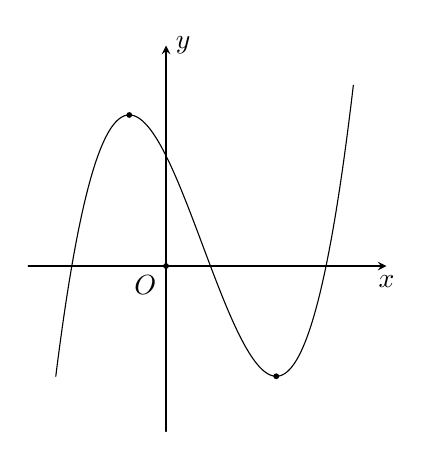
\begin{tikzpicture}[line join=round,line cap=round,>=stealth,scale=0.7,declare function={f(\x)=0.5*(\x)^3 - (\x)^2 - 2*(\x) + 2;}]
			\draw[->] (-2.5,0) -- (4,0) node[below] {$x$};
			\draw[->] (0,-3) -- (0,4) node[right] {$y$};
			\node at (0,0) [below left] {$O$};
			\draw[smooth,samples=500,domain=-2:3.4] plot (\x,{f(\x)});
			\fill  (-0.666,2.74) circle (1.5pt);
			\fill  (2,-2) circle (1.5pt);
			\fill (0,0) circle (1.5pt);
		\end{tikzpicture}
	}
	\loigiai{
		Dựa vào đồ thị hàm số $y=ax^3+bx^2+cx+d$, ta có các nhận xét sau
		\begin{itemize}
			\item $\lim\limits_{x\to +\infty}y=+\infty$ nên hệ số $a>0$.
			\item Đồ thị cắt trục tung tại điểm có tung độ dương (nằm phía trên trục hoành) nên hệ số tự do $d>0$.
			\item Hàm số có hai điểm cực trị $x_1$, $x_2$ trái dấu và nằm về hai phía trục tung.\\
			Ta có $y'=3ax^2+2bx+c$.\\
			Vì $x_1$, $x_2$ là nghiệm của phương trình $y'=0$ và $x_1x_2<0$ (trái dấu).\\
			Theo định lý Viète, ta được $x_1x_2=-\dfrac{c}{3a}<0$. Vì $a>0$ nên $c<0$.
			\item Quan sát hình vẽ, ta thấy điểm cực tiểu nằm xa gốc tọa độ hơn điểm cực đại (hoặc tổng hoành độ dương), tức là $x_1+x_2>0$.\\
			Theo định lý Viète, ta được $x_1+x_2=-\dfrac{2b}{3a}>0$. Vì $a>0$ nên $-2b>0\Leftrightarrow b<0$.
		\end{itemize}
		Vậy dấu của các hệ số là $a>0$, $b<0$, $c<0$, $d>0$.
	}
\end{ex}
%%%=============================%%%

%%%=============EX_7=============%%%
\begin{ex}%[1D2H3-4]%[TDMT05]%[Lê Phúc]
	Cho một cấp số nhân $\left(u_n\right)$ có công bội bằng số hạng đầu và số hạng thứ $4$ bằng $16$. Số hạng thứ hai của cấp số nhân này là
	\choice
	{$2$}
	{$32$}
	{$\dfrac{1}{8}$}
	{\True $4$}
	\loigiai{
		Ta có $u_1=q$.\\
		Lại có
		\begin{eqnarray*}
			u_4&=&16\\
			&\Leftrightarrow& u_1\cdot q^3=16\\
			&\Leftrightarrow& q\cdot q^3=16\\
			&\Leftrightarrow& q^4=16\\
			&\Leftrightarrow& q=2\ \left(\text{vì}\ u_4=16>0\right).
		\end{eqnarray*}
		Suy ra $u_1=2$.\\
		Số hạng thứ hai là $u_2=u_1\cdot q=2\cdot 2=4$.
	}
\end{ex}
%%%=============================%%%

%%%=============EX_8=============%%%
\begin{ex}%[0D8N2-2]%[TDMT05]%[Vũ Hồng Toàn]
	Số cách xếp $3$ người vào $7$ vị trí ghế hàng ngang là
	\choice
	{\True $210$}
	{$35$}
	{$21$}
	{$10$}
	\loigiai{
		Số cách xếp $3$ người vào $7$ vị trí ghế hàng ngang là số chỉnh hợp chập $3$ của $7$ phần tử.\\
		Vậy số cách xếp là $\mathrm{A}_7^3 = \dfrac{7!}{(7-3)!} = \dfrac{7!}{4!} = 210$.
	}
\end{ex}
%%%=============================%%%

%%%=============EX_9=============%%%
\begin{ex}%[1D6H4-3]%[TDMT05]%[Chu Ha]
	Tập nghiệm của bất phương trình $\left(\log_x x\right)\left(3^x-81\right)\leq0$ là
	\choice
	{$(0;4]$}
	{$(0;4)$}
	{\True $(0;1)\cup(1;4]$}
	{$(1;4)$}
	\loigiai{
		Điều kiện xác định $\heva{&x>0\\&x\neq 1.}$\\
		Với mọi $x$ thỏa mãn điều kiện xác định, ta luôn có $\log_x x=1$.\\
		Do đó bất phương trình đã cho tương đương với
		\begin{eqnarray*}
			&&\left(3^x-81\right)\leq0\\
			&\Leftrightarrow& 3^x-81\leq0\\
			&\Leftrightarrow& 3^x\leq81\\
			&\Leftrightarrow& x\leq4.
		\end{eqnarray*}
		Kết hợp điều kiện xác định $\heva{&x>0\\&x\neq 1}$, ta suy ra tập nghiệm của bất phương trình là $S=(0;1)\cup(1;4]$.
	}
\end{ex}
%%%=============================%%%

%%%=============EX_10=============%%%
\begin{ex}%[1H8H7-2]%[TDMT05]%[Nguyễn Sơn Thành]
	Cho hình chóp $S.ABCD$ có đáy là hình vuông cạnh bằng $3$, cạnh bên $SA$ vuông góc với đáy và $SA = 4$. Thể tích của khối chóp $S.ABC$ bằng
	\choice
	{$12$}
	{\True $6$}
	{$3$}
	{$9$}
	\loigiai{
		\immini{
			Đáy của khối chóp $S.ABC$ là tam giác $ABC$ vuông cân tại $B$.\\ Diện tích tam giác $ABC$ là
			\[S_{\triangle ABC} = \dfrac{1}{2} \cdot BA \cdot BC = \dfrac{1}{2} \cdot 3 \cdot 3 = \dfrac{9}{2}.\]
			Thể tích khối chóp $S.ABC$ là
			\[V_{S.ABC} = \dfrac{1}{3} \cdot S_{\triangle ABC} \cdot SA= \dfrac{1}{3} \cdot \dfrac{9}{2} \cdot 4 = 6.\]
		}{
			\begin{tikzpicture}[scale=1, font=\footnotesize, line join=round, line cap=round, >=stealth]
				\def\a{3}
				\path
				(0,0) coordinate (A)
				(0:\a) coordinate (D)
				(230:0.6*\a) coordinate (B)	
				($(D)+(B)$) coordinate (C)	
				(90:0.8*\a) coordinate (S);
				
				\draw (S)--(B)--(C)--(D)--(S)--(C);
				\draw[dashed] (S)--(A)--(B) (A)--(D) (A)--(C);
				
				\pic[draw,angle radius=2mm] {right angle = D--A--S};
				\pic[draw,angle radius=2mm] {right angle = A--B--C};
				
				\foreach \x/\g in {S/90,A/135,C/-45,B/-135,D/0}
				\fill[black] (\x) circle (1pt)+(\g:.3)node{$\x$};
			\end{tikzpicture}
		}
	}
\end{ex}
%%%=============================%%%

%%%=============EX_11=============%%%
\begin{ex}%[TDM21]%[2D1H4-1]
	Cho hàm số $f(x)$ có bảng biến thiên như hình vẽ. Số đường tiệm cận đứng và ngang của đồ thị hàm số $y = \dfrac{1}{f(x)}$ là
	\begin{center}
		
\begin{tikzpicture}
			\tkzTabInit[nocadre=false, lgt=1.2, espcl=2.5, deltacl=0.5]
			{$x$ /0.6, $f(x)$ /2}
			{$-\infty$, $-2$, $0$, $3$, $+\infty$}
			\tkzTabVar{-/ $2$, +/ $5$, -D+/ $-\infty$ / $+\infty$, -/ $-2$, +/ $+\infty$}
		\end{tikzpicture}
	\end{center}
	\choice
	{$6$}
	{\True $5$}
	{$4$}
	{$3$}
	\loigiai{
		Xét đồ thị hàm số $y = \dfrac{1}{f(x)}$.
		\begin{itemize}
			\item \textbf{Tiệm cận ngang:}
			Ta có $\lim\limits_{x \to +\infty} y = \lim\limits_{x \to +\infty} \dfrac{1}{f(x)} = 0$ (do $\lim\limits_{x \to +\infty} f(x) = +\infty$).\\
			$\lim\limits_{x \to -\infty} y = \lim\limits_{x \to -\infty} \dfrac{1}{f(x)} = \dfrac{1}{2}$ (do $\lim\limits_{x \to -\infty} f(x) = 2$).\\
			Suy ra đồ thị hàm số có $2$ đường tiệm cận ngang là $y=0$ và $y=\dfrac{1}{2}$.
			\item \textbf{Tiệm cận đứng:}
			Số đường tiệm cận đứng của đồ thị hàm số $y = \dfrac{1}{f(x)}$ là số nghiệm của phương trình $f(x) = 0$.\\
			Dựa vào bảng biến thiên, đường thẳng $y=0$ cắt đồ thị hàm số $y=f(x)$ tại $3$ điểm phân biệt (có hoành độ lần lượt thuộc các khoảng $(-2; 0)$, $(0; 3)$ và $(3; +\infty)$).\\
			Suy ra phương trình $f(x)=0$ có $3$ nghiệm phân biệt.\\
			Do đó, đồ thị hàm số có $3$ đường tiệm cận đứng.
		\end{itemize}
		Vậy đồ thị hàm số $y = \dfrac{1}{f(x)}$ có tất cả $2 + 3 = 5$ đường tiệm cận đứng và ngang.
	}
\end{ex}
%%%=============================%%%

%%%=============EX_12=============%%%
\begin{ex}%[TDM21]%[2H2H1-3]
	\immini[thm]{Cho hình lập phương $ABCD.A'B'C'D'$ có cạnh bằng $3$. Hãy tính giá trị của biểu thức $\left(\overrightarrow{AC'}+\overrightarrow{BD'}\right)\cdot\overrightarrow{AB}$.
		\choice
		{$9$}
		{$9\sqrt{2}$}
		{$3\sqrt{3}$}
		{\True $0$}}
	{\begin{tikzpicture}
			\def\a{3}
			\path 	(0:0) coordinate (A)
			++(0:\a) coordinate (D)
			++(-130:\a/2) coordinate (C)
			($(A)+(C)-(D)$) coordinate (B)
			($(A)+(90:\a)$) coordinate (A')
			($(B)+(90:\a)$) coordinate (B')
			($(C)+(90:\a)$) coordinate (C')
			($(D)+(90:\a)$) coordinate (D');
			\draw[dashed] 	(B)--(A)--(D)	(A)--(A');
			\draw	(C)--(C') 	(D)--(D') 	(B)--(B') 	(B)--(C)--(D) (A')--(B')--(C')--(D')--cycle;
			\foreach \x/\g in {A/135,B/180,C/-45,D/0,A'/135,B'/180,C'/-45,D'/0}
			\fill[black] 	(\x) circle (1pt)
			($(\g:3mm)+(\x)$) node {$\x$};	
		\end{tikzpicture}
	}
	\loigiai{
		Ta có:
		\begin{eqnarray*}
			\overrightarrow{AC'} + \overrightarrow{BD'} &=& \left(\overrightarrow{AB} + \overrightarrow{AD} + \overrightarrow{AA'}\right) + \left(\overrightarrow{BA} + \overrightarrow{BC} + \overrightarrow{BB'}\right) \\
			&=& \left(\overrightarrow{AB} + \overrightarrow{AD} + \overrightarrow{AA'}\right) + \left(-\overrightarrow{AB} + \overrightarrow{AD} + \overrightarrow{AA'}\right) \\
			&=& 2\overrightarrow{AD} + 2\overrightarrow{AA'}.
		\end{eqnarray*}
		Khi đó:
		\begin{eqnarray*}
			\left(\overrightarrow{AC'} + \overrightarrow{BD'}\right) \cdot \overrightarrow{AB} &=& \left(2\overrightarrow{AD} + 2\overrightarrow{AA'}\right) \cdot \overrightarrow{AB} \\
			&=& 2\overrightarrow{AD} \cdot \overrightarrow{AB} + 2\overrightarrow{AA'} \cdot \overrightarrow{AB}.
		\end{eqnarray*}
		Vì $ABCD.A'B'C'D'$ là hình lập phương nên $AD \perp AB$ và $AA' \perp AB$.\\
		Suy ra $\overrightarrow{AD} \cdot \overrightarrow{AB} = 0$ và $\overrightarrow{AA'} \cdot \overrightarrow{AB} = 0$.\\
		Vậy $\left(\overrightarrow{AC'} + \overrightarrow{BD'}\right) \cdot \overrightarrow{AB} = 0$.
	}
\end{ex}
%%%=============================%%%
\Closesolutionfile{ans}

\cauds
\Opensolutionfile{ans}[ans/ansTN-DungSai]
%%%=============EX_13=============%%%
\begin{ex}%[2D1H3-2]%[TDMT05]%[Dương Công Tạo]
	Cho hàm số $f(x) = 4x - \tan x$, xét trên khoảng $\left( -\dfrac{\pi}{2}; \dfrac{\pi}{2} \right)$.
	\choiceTF[t]
	{\True $f'(x) = 4 - \dfrac{1}{\cos^2 x}$, $x \in \left( -\dfrac{\pi}{2}; \dfrac{\pi}{2} \right)$}
	{$f'(x) = 0 \Leftrightarrow x = \dfrac{\pi}{3}$}
	{\True $f\left( -\dfrac{\pi}{3} \right) = -\dfrac{4\pi}{3} + \sqrt{3}$; $f\left( \dfrac{\pi}{3} \right) = \dfrac{4\pi}{3} - \sqrt{3}$}
	{$\displaystyle \min_{\left( -\tfrac{\pi}{2}; \tfrac{\pi}{2} \right)} f(x) = f\left( -\dfrac{\pi}{3} \right)$}
	\loigiai{
		\begin{itemchoice}
			\itemch Xét hàm số $f(x) = 4x - \tan x$, trên khoảng $\left( -\dfrac{\pi}{2}; \dfrac{\pi}{2} \right)$.\\
			Ta có $f'(x) = 4-\dfrac{1}{\cos^2x}$, $\forall x\in\left( -\dfrac{\pi}{2}; \dfrac{\pi}{2} \right)$.
			\itemch $f'(x)= 4-\dfrac{1}{\cos^2x}=4-\left(1+\tan^2x\right)=3-\tan^2x$, $\forall x\in\left( -\dfrac{\pi}{2}; \dfrac{\pi}{2} \right)$.\\
			$f'(x)=0\Leftrightarrow 3-\tan^2x=0\Leftrightarrow \tan x=\pm\sqrt{3}\Leftrightarrow x=\pm \dfrac{\pi}{3}$.
			\itemch Với $f(x) = 4x - \tan x$, ta có
			\begin{itemize}
				\item $f\left(-\dfrac{\pi}{3}\right)=4\cdot\left(-\dfrac{\pi}{3}\right)-4\cdot\tan\left(-\dfrac{\pi}{3}\right)= -\dfrac{4\pi}{3} + \sqrt{3}$;
				\item $f\left(\dfrac{\pi}{3}\right)=4\cdot\dfrac{\pi}{3}-4\cdot\tan\dfrac{\pi}{3}=\dfrac{4\pi}{3} - \sqrt{3}$.
			\end{itemize}
			\itemch Xét hàm số $f(x) = 4x - \tan x$, trên khoảng $\left( -\dfrac{\pi}{2}; \dfrac{\pi}{2} \right)$.\\
			Ta có $f'(x) = 4-\dfrac{1}{\cos^2x}=3-\tan^2x$, $\forall x\in\left( -\dfrac{\pi}{2}; \dfrac{\pi}{2} \right)$.\\
			$f'(x)=0\Leftrightarrow 3-\tan^2x=0\Leftrightarrow \tan x=\pm\sqrt{3}\Leftrightarrow x=\pm \dfrac{\pi}{3}$.\\
			Bảng biến thiên
			\begin{center}
				
\begin{tikzpicture}[>=stealth]
					\tkzTabInit[nocadre=false,lgt=1.5,espcl=3,deltacl=0.6]{$x$/.7 ,$f'(x)$/.7,$f(x)$/2}
					{$-\tfrac{\pi}{2}$ , $-\tfrac{\pi}{3}$ , $\tfrac{\pi}{3}$ , $\tfrac{\pi}{2}$}
					\tkzTabLine{ , - , $0$ ,+ , $0$ , - , }
					\tkzTabVar{+/$+\infty$ , -/$-\dfrac{4\pi}{3} + \sqrt{3}$ , +/$\dfrac{4\pi}{3} - \sqrt{3}$ , -/$-\infty$}
				\end{tikzpicture}
			\end{center}
			Dựa vào bảng biến thiên, ta thấy hàm số đã cho không tồn tại giá trị nhỏ nhất và giá trị lớn nhất trên khoảng $\left( -\dfrac{\pi}{2}; \dfrac{\pi}{2} \right)$.
		\end{itemchoice}
	}
\end{ex}
%%%=============================%%%

%%%=============EX_14=============%%%
\begin{ex}%[2D1H3-4]%[TDMT05]%[Nguyễn Tấn Linh]
	Cho hàm số $f(x) = x^2 - 2026\ln x$.
	\choiceTF[t]
	{\True Tập xác định của hàm số là $(0; +\infty)$}
	{\True $f'(x) = 2x - \dfrac{2026}{x}$}
	{\True $\min\limits_{x\in\mathscr{D}} f(x) = f\left(\sqrt{1013}\right)$}
	{\True Có tất cả $95$ giá trị nguyên của $x$ để $f(x)$ nhận giá trị âm}
	\loigiai
	{
		\begin{itemchoice}
			\itemch Điều kiện xác định là $x > 0$. Vậy tập xác định của hàm số là $\mathscr{D} = (0; +\infty)$.
			\itemch Ta có đạo hàm $f'(x) = \left(x^2\right)' - 2026(\ln x)' = 2x - 2026 \cdot \dfrac{1}{x} = 2x - \dfrac{2026}{x}$.
			\itemch Xét phương trình
			\[f'(x) = 0 \Leftrightarrow 2x - \dfrac{2026}{x} = 0 \Rightarrow 2x^2 = 2026 \Leftrightarrow x^2 = 1013\Leftrightarrow \hoac{& x=\sqrt{1013} \\ & x=-\sqrt{1013}.}\]
			Vì $x \in \mathscr{D}$ nên ta nhận nghiệm $x = \sqrt{1013}$.\\
			Dễ thấy $f'(x)$ đổi dấu từ âm sang dương khi qua điểm $x = \sqrt{1013}$ nên hàm số đạt cực tiểu tại điểm này.\\
			Vì trên khoảng $(0; +\infty)$ hàm số chỉ có một điểm cực trị duy nhất là điểm cực tiểu nên giá trị cực tiểu cũng là giá trị nhỏ nhất của hàm số trên tập xác định.\\
			Vậy $\min\limits_{x\in\mathscr{D}} f(x) = f\left(\sqrt{1013}\right)$.
			\itemch Bảng biến thiên của hàm số:
			\begin{center}
				
\begin{tikzpicture}
					\tkzTabInit[nocadre=false,lgt=1.2,espcl=3,deltacl=0.6]
					{$x$ /0.7,$f'(x)$ /0.7,$f(x)$ /2}
					{$0$,$\sqrt{1013}$,$+\infty$}
					\tkzTabLine{d,-,0,+,}
					\tkzTabVar{D+/$+\infty$,-/$f\left(\sqrt{1013}\right)<0$,+/$+\infty$}
				\end{tikzpicture}
			\end{center}
			Dựa vào bảng biến thiên, ta thấy phương trình $f(x)=0$ có hai nghiệm phân biệt.\\
			Hàm số $f(x)$ liên tục trên khoảng $(0; +\infty)$.
			\begin{itemize}
				\item Trên khoảng $(1; 2)$, hàm số nghịch biến.\\ Ta có
				$\heva{& f(1) = 1 > 0 \\ & f(2) = 4 - 2026\ln 2 \approx -1400{,}3 < 0} \Rightarrow f(1) \cdot f(2) < 0$.\\
				Suy ra phương trình có duy nhất một nghiệm $x_1 \in (1; 2)$.
				\item Trên khoảng $(96; 97)$, hàm số đồng biến.\\ Ta có:
				$\heva{& f(96) = 96^2 - 2026\ln 96 \approx -31{,}3 < 0 \\ & f(97) = 97^2 - 2026\ln 97 \approx 140{,}7 > 0} \Rightarrow f(96) \cdot f(97) < 0$.\\
				Suy ra phương trình có duy nhất một nghiệm $x_2 \in (96; 97)$.
			\end{itemize}
			Dựa vào bảng biến thiên, $f(x) < 0\Leftrightarrow x_1 < x < x_2$.\\
			Vì $x$ là số nguyên nên $x \in \{2; 3; \ldots; 96\}$.\\
			Số các giá trị nguyên thỏa mãn là $96 - 2 + 1 = 95$.
		\end{itemchoice}
	}
\end{ex}
%%%=============================%%%

\begin{ex}%[2H2V1-4]
	\immini[thm]{
		Cho hình chóp đều $S. ABCD$ có chiều dài cạnh đáy bằng $6$ cm và cạnh bên bằng $8$ cm. Tâm của đáy là điểm $O$.
		\choiceTF[t]
		{\True $\overrightarrow{SA} + \overrightarrow{SB} + \overrightarrow{SC} + \overrightarrow{SD} = 4\overrightarrow{SO}$}
		{$\overrightarrow{SC} \cdot \overrightarrow{CD} = 18$}
		{\True $\left(\overrightarrow{SB} + \overrightarrow{SC}\right) \cdot \left(\overrightarrow{DC} + \overrightarrow{DA}\right) = 36$}
		{Ở cùng một thời điểm chú kiến $X$ bắt đầu bò từ $A$ đến $B$, chú kiến $Y$ bắt đầu bò từ $C$ đến $S$, cả hai bò với tốc độ không đổi bằng $1$ cm/s. Khoảng cách ngắn nhất của hai chú kiến này là $5{,}81$ cm (\textit{tính theo centimet và làm tròn kết quả đến hàng phần trăm})}
	}{
		\begin{tikzpicture}[scale=1, font=\footnotesize, line join=round, line cap=round,>=stealth]
			\path
			(0,0) coordinate (A)
			(-1.9,-1.6)coordinate (B)
			(1.6,-1.6)coordinate (C)
			($(A)+(C)-(B)$)coordinate (D)
			($(A)!0.5!(C)$)coordinate (O)
			($(O)+(0,3.5)$) coordinate (S)
			;
			\draw (S)--(B)--(C)--(D)--cycle (S)--(C);
			\draw[dashed] (O)--(S)--(A)--(D) (C)--(A)--(B)--(D);	
			\foreach \p/\q in {S/90,A/180,B/-90,C/-90,D/0,O/-90}
			\fill[black] (\p) circle (1.0pt)node[shift={(\q:3mm)}]{$\p$};		
		\end{tikzpicture}
	}
	\loigiai{
		\begin{center}
			\begin{tikzpicture}[scale=1, font=\footnotesize, line join=round, line cap=round,>=stealth]
				\path
				(0,0) coordinate (A)
				(-1.9,-1.6)coordinate (B)
				(1.6,-1.6)coordinate (C)
				($(A)+(C)-(B)$)coordinate (D)
				($(A)!0.5!(C)$)coordinate (O)
				($(O)+(0,3.5)$) coordinate (S)
				($(A)!0.4!(B)$)coordinate (M)
				($(C)!0.45!(S)$)coordinate (N)
				;
				\draw (S)--(B)--(C)--(D)--cycle (S)--(C);
				\draw[dashed] (O)--(S)--(A)--(D) (C)--(A)--(B)--(D) (M)--(N);	
				\foreach \p/\q in {S/90,A/180,B/-90,C/-90,D/0,O/-90,M/140,N/50}
				\fill[black] (\p) circle (1.0pt)node[shift={(\q:3mm)}]{$\p$};		
			\end{tikzpicture}
		\end{center}
		\begin{itemchoice}
			\itemch Ta có $O$ là trung điểm của $AC$ và $BD$ nên
			$\heva{&\overrightarrow{SA} + \overrightarrow{SC} = 2\overrightarrow{SO}\\&\overrightarrow{SB} + \overrightarrow{SD} = 2\overrightarrow{SO}}\Rightarrow \overrightarrow{SA} +\overrightarrow{SB} +\overrightarrow{SC} +\overrightarrow{SD}=4\overrightarrow{SO}$.
			\itemch Ta có $\overrightarrow{SC} \cdot \overrightarrow{SD}=\dfrac{SC^2+SD^2-CD^2}{2}=\dfrac{8^2+8^2-6^2}{2}=46$.\\
			Do đó $\overrightarrow{SC} \cdot \overrightarrow{CD}=\overrightarrow{SC}\cdot\left(\overrightarrow{SD}-\overrightarrow{SC}\right) = \overrightarrow{SC} \cdot \overrightarrow{SD} - SC^2 = 46 - 64 = -18$.
			\itemch Ta có $\overrightarrow{DC} + \overrightarrow{DA} = \overrightarrow{DB}$.\\
			Khi đó $P = \left(\overrightarrow{SB} + \overrightarrow{SC}\right) \cdot \overrightarrow{DB} = \left(\overrightarrow{SO} + \overrightarrow{OB} + \overrightarrow{SO} + \overrightarrow{OC}\right) \cdot \overrightarrow{DB} = \left(2\overrightarrow{SO} + \overrightarrow{OB} + \overrightarrow{OC}\right) \cdot \overrightarrow{DB}$.\\
			Vì $S.ABCD$ là chóp đều nên $SO \perp (ABCD) \Rightarrow \overrightarrow{SO} \cdot \overrightarrow{DB} = 0$.\\
			Đáy $ABCD$ là hình vuông nên $AC \perp BD \Rightarrow \overrightarrow{OC} \cdot \overrightarrow{DB} = 0$.\\
			Suy ra $P = \overrightarrow{OB} \cdot \overrightarrow{DB} = \dfrac{1}{2}\overrightarrow{DB} \cdot \overrightarrow{DB} = \dfrac{1}{2}DB^2$.\\
			Với $AB=6$, ta có $DB = 6\sqrt{2}$.\\ Vậy $P = \dfrac{1}{2} \cdot \left(6\sqrt{2}\right)^2 = 36$.
			\itemch Gọi $t$ là thời gian ($0 \leq t \leq 6$).\\ Vị trí kiến là $M \in AB$, $N \in CS$ với $AM=CN=t$. \\
			Suy ra $\overrightarrow{AM}=\dfrac{t}{6}\overrightarrow{AB}$.\\ $\overrightarrow{CN}=\dfrac{t}{8}\overrightarrow{CS}\Leftrightarrow \overrightarrow{AN}-\overrightarrow{AC}
			=\dfrac{t}{8}\left(\overrightarrow{AS}-\overrightarrow{AC}\right)\Leftrightarrow \overrightarrow{AN} =\dfrac{t}{8}\overrightarrow{AS}+\dfrac{-t+8}{8}\overrightarrow{AB} +\dfrac{-t+8}{8}\overrightarrow{AD}$.\\
			Ta có $\overrightarrow{AB}\cdot \overrightarrow{AD}=0$, $\overrightarrow{AD}\cdot \overrightarrow{AS}= \overrightarrow{AB}\cdot \overrightarrow{AS}= \dfrac{AB^2+AS^2-SB^2}{2}=\dfrac{6^2+8^2-8^2}{2}=18$.
			\begin{eqnarray*}
				MN^2&=&\left(\overrightarrow{AN}-\overrightarrow{AM}\right)^2\\
				&=&\left(\dfrac{t}{8}\overrightarrow{AS}+\dfrac{-7t+24}{24}\overrightarrow{AB} +\dfrac{-t+8}{8}\overrightarrow{AD}\right)^2\\
				&=&\left(\dfrac{t}{8}\right)^2\cdot8^2+\left(\dfrac{-7t+24}{24}\right)^2\cdot 6^2 +\left(\dfrac{-t+8}{8}\right)^2\cdot 6^2 +2\cdot\dfrac{t}{8}\cdot\dfrac{-7t+24}{24}\cdot18+2\cdot\dfrac{t}{8}\cdot\dfrac{-t+8}{8}\cdot18\\
				&=& \dfrac{11}{4}t^2 -21t+72
				=\dfrac{11}{4}\left(t-\dfrac{42}{11}\right)^2+\dfrac{351}{11}\\
				&\ge&\dfrac{351}{11}.
			\end{eqnarray*}
			Giá trị nhỏ nhất $MN = \sqrt{\dfrac{351}{11}} \approx 5{,}65$ cm khi $t=\dfrac{42}{11}$.
		\end{itemchoice}
	}
\end{ex}

%%%=============EX_16=============%%%
\begin{ex}%[0D0V2-6]%[TDMT05]%[Hà Văn Hảo]
	\immini[thm]{Cho $9$ ô vuông nhỏ được xếp sát với nhau tạo thành một hình vuông lớn như hình vẽ. Một em bé cầm trong tay $5$ hạt đậu để đặt ngẫu nhiên vào $9$ ô vuông nhỏ này, sao cho mỗi ô vuông nhỏ chỉ có tối đa một hạt đậu.}{
		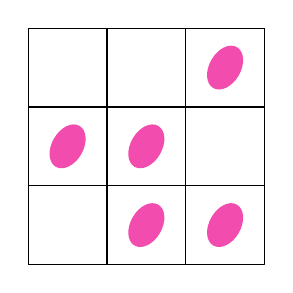
\begin{tikzpicture}[line cap=round, line join=round,font=\footnotesize]
			\def\a{1}
			\foreach \x in{1,2,3}{\draw (0,0) rectangle (\x*\a,\x*\a);\draw (0,1) rectangle (\x*\a,2*\a);\draw (0,2) rectangle (\x*\a,3*\a);}	
			\tikzset{keo/.pic={
					\begin{scope}[rotate=60]
						\fill[ color=magenta!70] (0,0) ellipse ({0.3} and {0.2});
					\end{scope}
			}}
			\pic at(2+\a/2,2+\a/2) {keo};
			\foreach \x in{1,2}{\pic at(\a/2+\x,\a/2) {keo};}	
			\foreach \x in{0,1}{\pic at(\a/2+\x,1+\a/2) {keo};}
		\end{tikzpicture}
	}
	\choiceTF[t]
	{\True Em bé có tất cả $126$ cách đặt các hạt đậu vào $9$ ô vuông}
	{\True Có $4$ cách để sau khi đặt $5$ hạt đậu vào sẽ cho ta $5$ ô đặt hạt đậu tạo thành hình chữ T}
	{\True Có $4$ cách để sau khi đặt $5$ hạt đậu vào sẽ cho ta $4$ ô trống ghép thành một hình vuông}
	{\True Xác suất để bất kì hàng nào hoặc cột nào tạo thành từ $9$ ô vuông đều có hạt đậu là $\dfrac{5}{7}$}
	\loigiai{
		Số phần tử của không gian mẫu là số cách chọn $5$ ô từ $9$ ô để đặt hạt đậu
		$ n(\Omega) = \mathrm{C}_9^5 = 126$.
		\begin{itemchoice}
			\itemch Em bé có số cách đặt hạt đậu là $\mathrm{C}_9^5 = 126$ cách.
			\itemch Một hình chữ T cấu tạo từ $5$ ô vuông trong lưới $3 \times 3$ có thể xoay theo $4$ hướng (T thuận hướng lên, T ngược hướng xuống, T xoay qua trái, T xoay qua phải). Mỗi hướng chỉ có duy nhất $1$ vị trí đặt để không bị tràn ra ngoài lưới $3 \times 3$.\\
			Vậy có $4$ cách.
			\begin{center}
				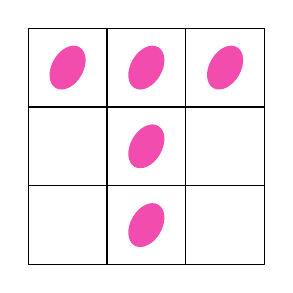
\begin{tikzpicture}[line cap=round, line join=round,font=\footnotesize]
					\def\a{1}
					\foreach \x in{1,2,3}{\draw (0,0) rectangle (\x*\a,\x*\a);\draw (0,1) rectangle (\x*\a,2*\a);\draw (0,2) rectangle (\x*\a,3*\a);}	
					\tikzset{keo/.pic={
							\begin{scope}[rotate=60]
								\fill[ color=magenta!70] (0,0) ellipse ({0.3} and {0.2});
							\end{scope}
					}}
					\foreach \x in{0,1}{\pic at(1+\a/2,\x+\a/2) {keo};}	
					\foreach \x in{0,1,2}{\pic at(\a/2+\x,2+\a/2) {keo};}
				\end{tikzpicture}
				\hspace{1 cm}
				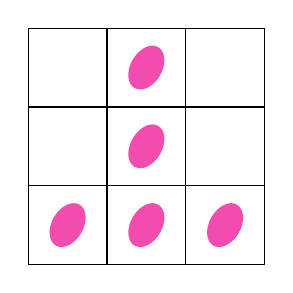
\begin{tikzpicture}[line cap=round, line join=round,font=\footnotesize]
					\def\a{1}
					\foreach \x in{1,2,3}{\draw (0,0) rectangle (\x*\a,\x*\a);\draw (0,1) rectangle (\x*\a,2*\a);\draw (0,2) rectangle (\x*\a,3*\a);}	
					\tikzset{keo/.pic={
							\begin{scope}[rotate=60]
								\fill[ color=magenta!70] (0,0) ellipse ({0.3} and {0.2});
							\end{scope}
					}}
					\foreach \x in{1,2}{\pic at(\a/2+1,\a/2+\x) {keo};}	
					\foreach \x in{0,1,2}{\pic at(\a/2+\x,\a/2) {keo};}
				\end{tikzpicture}
				\hspace{1 cm}
				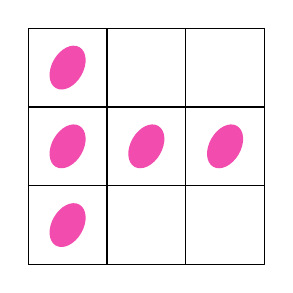
\begin{tikzpicture}[line cap=round, line join=round,font=\footnotesize]
					\def\a{1}
					\foreach \x in{1,2,3}{\draw (0,0) rectangle (\x*\a,\x*\a);\draw (0,1) rectangle (\x*\a,2*\a);\draw (0,2) rectangle (\x*\a,3*\a);}	
					\tikzset{keo/.pic={
							\begin{scope}[rotate=60]
								\fill[ color=magenta!70] (0,0) ellipse ({0.3} and {0.2});
							\end{scope}
					}}
					\foreach \x in{1,2}{\pic at(\a/2+\x,1+\a/2) {keo};}	
					\foreach \x in{0,1,2}{\pic at(\a/2,\x+\a/2) {keo};}
				\end{tikzpicture}
				\hspace{1 cm}
				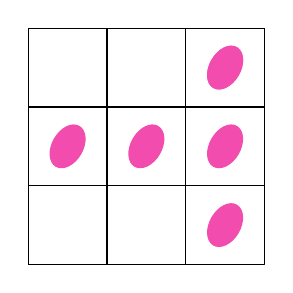
\begin{tikzpicture}[line cap=round, line join=round,font=\footnotesize]
					\def\a{1}
					\foreach \x in{1,2,3}{\draw (0,0) rectangle (\x*\a,\x*\a);\draw (0,1) rectangle (\x*\a,2*\a);\draw (0,2) rectangle (\x*\a,3*\a);}	
					\tikzset{keo/.pic={
							\begin{scope}[rotate=60]
								\fill[ color=magenta!70] (0,0) ellipse ({0.3} and {0.2});
							\end{scope}
					}}
					\pic at(2+\a/2,2+\a/2) {keo};
					\foreach \x in{0,1}{\pic at(\a/2+\x,1+\a/2) {keo};}	
					\foreach \x in{0,1,2}{\pic at(2+\a/2,\x+\a/2) {keo};}
				\end{tikzpicture}
			\end{center}
			\itemch Để $4$ ô trống tạo thành một hình vuông, thì $4$ ô đó phải tạo thành một khối $2 \times 2$. Trong lưới $3 \times 3$, có đúng $4$ vị trí cho khối $2 \times 2$ (tương ứng với các góc của hình vuông lớn).\\
			Vậy có $4$ cách để $4$ ô trống tạo thành hình vuông.
			\begin{center}
				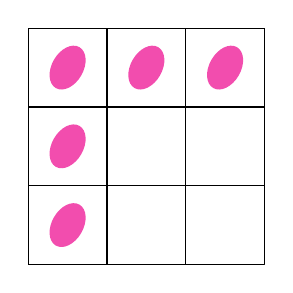
\begin{tikzpicture}[line cap=round, line join=round,font=\footnotesize]
					\def\a{1}
					\foreach \x in{1,2,3}{\draw (0,0) rectangle (\x*\a,\x*\a);\draw (0,1) rectangle (\x*\a,2*\a);\draw (0,2) rectangle (\x*\a,3*\a);}	
					\tikzset{keo/.pic={
							\begin{scope}[rotate=60]
								\fill[ color=magenta!70] (0,0) ellipse ({0.3} and {0.2});
							\end{scope}
					}}
					\foreach \x in{0,1}{\pic at(\a/2,\x+\a/2) {keo};}	
					\foreach \x in{0,1,2}{\pic at(\a/2+\x,2+\a/2) {keo};}
				\end{tikzpicture}
				\hspace{1 cm}
				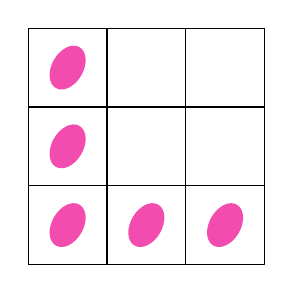
\begin{tikzpicture}[line cap=round, line join=round,font=\footnotesize]
					\def\a{1}
					\foreach \x in{1,2,3}{\draw (0,0) rectangle (\x*\a,\x*\a);\draw (0,1) rectangle (\x*\a,2*\a);\draw (0,2) rectangle (\x*\a,3*\a);}	
					\tikzset{keo/.pic={
							\begin{scope}[rotate=60]
								\fill[ color=magenta!70] (0,0) ellipse ({0.3} and {0.2});
							\end{scope}
					}}
					\foreach \x in{1,2}{\pic at(\a/2,\a/2+\x) {keo};}	
					\foreach \x in{0,1,2}{\pic at(\a/2+\x,\a/2) {keo};}
				\end{tikzpicture}
				\hspace{1 cm}
				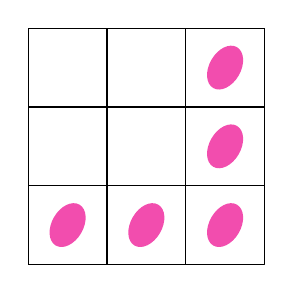
\begin{tikzpicture}[line cap=round, line join=round,font=\footnotesize]
					\def\a{1}
					\foreach \x in{1,2,3}{\draw (0,0) rectangle (\x*\a,\x*\a);\draw (0,1) rectangle (\x*\a,2*\a);\draw (0,2) rectangle (\x*\a,3*\a);}	
					\tikzset{keo/.pic={
							\begin{scope}[rotate=60]
								\fill[ color=magenta!70] (0,0) ellipse ({0.3} and {0.2});
							\end{scope}
					}}
					\foreach \x in{1,2}{\pic at(2+\a/2,\x+\a/2) {keo};}	
					\foreach \x in{0,1,2}{\pic at(\x+\a/2,\a/2) {keo};}
				\end{tikzpicture}
				\hspace{1 cm}
				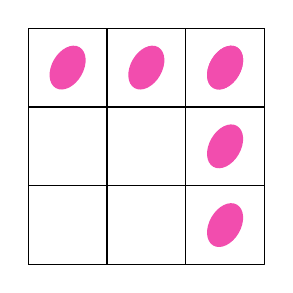
\begin{tikzpicture}[line cap=round, line join=round,font=\footnotesize]
					\def\a{1}
					\foreach \x in{1,2,3}{\draw (0,0) rectangle (\x*\a,\x*\a);\draw (0,1) rectangle (\x*\a,2*\a);\draw (0,2) rectangle (\x*\a,3*\a);}	
					\tikzset{keo/.pic={
							\begin{scope}[rotate=60]
								\fill[ color=magenta!70] (0,0) ellipse ({0.3} and {0.2});
							\end{scope}
					}}
					\pic at(2+\a/2,2+\a/2) {keo};
					\foreach \x in{0,1}{\pic at(\a/2+\x,2+\a/2) {keo};}	
					\foreach \x in{0,1,2}{\pic at(2+\a/2,\x+\a/2) {keo};}
				\end{tikzpicture}
			\end{center}
			\itemch	Gọi $A$ là biến cố: \lq\lq Mọi hàng và mọi cột đều có ít nhất một hạt đậu\rq\rq.\\
			Ta xét biến cố đối $\overline{A}$: \lq\lq Có ít nhất một hàng hoặc một cột không có hạt đậu nào\rq\rq.\\
			Vì chỉ có $5$ hạt đậu nên tối đa chỉ có thể có $1$ hàng trống hoặc $1$ cột trống.
			\begin{itemize}
				\item Số cách chọn $1$ hàng trống có $\mathrm{C}_3^1$ cách chọn hàng, sau đó chọn $5$ ô từ $6$ ô còn lại
				\[\mathrm{C}_3^1 \cdot \mathrm{C}_6^5 = 3 \cdot 6 = 18 \text{ cách.}\]
				\item Số cách chọn $1$ cột trống, tương tự có $\mathrm{C}_3^1 \cdot \mathrm{C}_6^5 = 18$ cách.\\
				\textit{Lưu ý}: Không có trường hợp vừa có hàng trống vừa có cột trống mà vẫn đặt đủ $5$ hạt đậu (vì nếu trống $1$ hàng và $1$ cột thì chỉ còn $4$ ô trống, không đủ chỗ cho $5$ hạt).
				\item Số phần tử của biến cố đối là $ n(\overline{A}) = 18 + 18 = 36$ cách.
				\item Số phần tử của biến cố $A$ là	$ n(A) = 126 - 36 = 90$ cách.
			\end{itemize}
			Vậy xác suất của biến cố $A$ là	$ \mathrm{P}(A) = \dfrac{90}{126} = \dfrac{5}{7}$.
		\end{itemchoice}
	}
\end{ex}
%%%=============================%%%
\Closesolutionfile{ans}

\caukq
\Opensolutionfile{ans}[ans/ansTN-DienKhuyet]
%%%=============EX_17=============%%%
\begin{ex}%[1H8H7-6]%[TDMT05]%[Lê Hồ Quang Minh]
	Cho khối chóp cụt tứ giác đều có độ dài hai cạnh đáy là $6$ và $8$, có góc giữa cạnh bên và đáy bằng $60^\circ$. Hãy tính thể tích của khối chóp cụt đều này \textit{(làm tròn kết quả đến hàng đơn vị).}
	\par
	\shortans[0]{121}
	\loigiai{
		\immini{
			Gọi $O$, $O'$ lần lượt là tâm của hai mặt đáy.\\
			Suy ra $OO'$ là chiều cao của khối chóp cụt đều $ABCD. A'B'C'D'$.\\
			Gọi $H$ là hình chiếu của $C'$ trên mặt phẳng $(ABCD)$.\\
			Suy ra $H \in AC$ và góc giữa $C'C$ với mặt phẳng đáy là $\big(C'C, (ABCD)\big)= \widehat{C'CH}$.\\
			Theo giả thiết ta có $\widehat{C'CH} = 60^\circ$.\\
			Mặt khác, $ABCD$ là hình vuông cạnh $8$ và $A'B'C'D'$ là hình vuông cạnh $6$ nên $\heva{&AC=8\sqrt{2}\\ &A'C'=6\sqrt{2}.}$\\
			Suy ra $HC=\dfrac{AC-A'C'}{2}=\sqrt{2}$.\\
			Khi đó $OO'=C'H=HC\cdot \tan 60^\circ=\sqrt{6}$.\\
			Vậy thể tích khối chóp cụt đều là 
			\[V=\dfrac{1}{3}\cdot OO' \cdot \left(S_{ABCD}+ S_{A'B'C'D'} + \sqrt{S_{ABCD}\cdot S_{A'B'C'D'}}\right)=\dfrac{1}{3}\cdot \sqrt{6} \cdot \left(64+36+48\right)=\dfrac{148\sqrt{6}}{3} \approx 121.\]
		}{
			\begin{tikzpicture}[declare function={h=3; rx=3; ry=1.2; rxp=2; ryp=0.8;}, font=\footnotesize, line join=round, line cap=round, >=stealth, scale=0.9]
				\coordinate (O) at (0,0);
				\coordinate (O') at (0,h);
				\path ($(O)+(105:rx and ry)$) coordinate (A)
				($(O)+(190:rx and ry)$) coordinate (B)
				($(A)!2!(O)$) coordinate (C)
				($(B)!2!(O)$) coordinate (D);
				\path ($(O')+(105:rxp and ryp)$) coordinate (A')
				($(O')+(190:rxp and ryp)$) coordinate (B')
				($(A')!2!(O')$) coordinate (C')
				($(B')!2!(O')$) coordinate (D');
				\coordinate (H) at ($(O)!2/3!(C)$);
				
				\draw[dashed] (A)--(D) (A)--(B) (A)--(A') (A)--(C) (O')--(O) (C')--(H) (B)--(D); 
				\draw (B)--(C)--(D) node[midway,rotate=32,below]{$8$} (A')--(B')--(C')--(D')--(A') node[midway,rotate=-14,above]{$6$} (B)--(B') (C)--(C') (D)--(D') (A')--(C'); 
				
				\path pic[draw,angle radius=5pt] {right angle = O'--O--C};
				\path pic[draw,angle radius=5pt] {right angle = C'--H--C};
				
				\foreach \x/\g in {A/150, B/180, C/-90, D/-30, A'/90, B'/180, C'/-15, D'/0, O'/15, O/-120, H/-170} 
				\filldraw (\x) circle (1pt) node[shift={(\g:3mm)}]{$\x$}; 
			\end{tikzpicture}
		}
	}
\end{ex}
%%%=============================%%%

%%%=============EX_18=============%%%
\begin{ex}%[0D3V2-6]%[TDMT05]%[Lương Pho]
		Bác Hùng chỉ có $45$ mét chiều dài hàng rào để quây thành hai ô để chăn nuôi ở bờ sông. Người này thiết kế hình dạng hàng rào như hình vẽ gồm một đoạn song song với bờ sông, ba đoạn bằng nhau song song với nhau và vuông góc với bờ sông. Hãy tính theo mét vuông, tổng diện tích lớn nhất mà bác Hùng quây được (\textit{làm tròn kết quả đến hàng đơn vị}).
	
	\begin{center}
			\begin{tikzpicture}[scale=1, font=\footnotesize, line join=round, line cap=round, >=stealth]
			\fill[white!80!green] (-1,-0.5) rectangle (12.5,2);
			\fill[white!70!cyan] (-1,2) rectangle (12.5,3);
			\fill[white!90!brown] (0,0)--(10,0)--(11.8,2)--(1.8,2)--cycle;
			
			\tikzset{tru/.pic={
					\shade[top color=brown, bottom color=brown!50, shading angle={100}, fill=brown!70, rounded corners=0.5ex, thick] (0:0)--++(90:0.8)--++(60:0.2)--++(-60:0.2)--++(-90:0.8)--cycle;
					\draw[fill=black!50] (0.1,0.6) circle (0.2mm);	
			}}
			\draw[line width=1mm,brown!50] (0,0.6)--(10,0.6);
			\draw[line width=1mm,brown!50] (0,0)--(10.2,0);
			\foreach \x in {0,1,...,25} {\pic at (0.4*\x,0) {tru};}
			
			\tikzset{cot/.pic={
					\shade[top color=brown, bottom color=brown!50, shading angle={100}, fill=brown!70, rounded corners=0.5ex, thick] (0:0)--++(90:0.75)--++(60:0.1)--++(-60:0.1)--++(-90:0.75)--cycle;
			}}
			\draw[line width=0.5mm,brown!50] (0,2)--(12.5,2);
			\draw[line width=1mm,brown!50] (0,0)--(1.8,2) (0,0.55)--(1.8,2.55);
			\draw[line width=1mm,brown!50] (5,0)--(6.8,2) (5,0.55)--(6.8,2.55);
			\draw[line width=1mm,brown!50] (10,0)--(11.8,2) (10,0.55)--(11.8,2.55);
			
			\foreach \x in {0,0.5,...,5} {
				\pic at (0.35*\x,0.4*\x) {cot};
				\pic at ($(5,0)+(0.35*\x,0.4*\x)$) {cot};
				\pic at ($(10,0)+(0.35*\x,0.4*\x)$) {cot};
			}			
		\end{tikzpicture}
	
	\end{center}
	\par
	\shortans[0]{169}
	\loigiai{
		Gọi $x$ (m) là chiều dài của mỗi đoạn hàng rào vuông góc với bờ sông ($x > 0$).\\
		Gọi $y$ (m) là chiều dài của đoạn hàng rào song song với bờ sông ($y > 0$).\\
		Theo giả thiết, tổng chiều dài hàng rào là $45\mathrm{\,m}$, nên ta có
		\[3x+y=45 \Rightarrow y=45-3x.\]
		Điều kiện $45-3x > 0 \Leftrightarrow 0 < x < 15$.\\
		Tổng diện tích của hai ô đất là
		\[S=x \cdot y=x(45-3x)=-3x^2+45x.\]
		Xét hàm số $f(x)=-3x^2+45x$ trên khoảng $(0; 15)$.\\
		Hàm số đạt giá trị lớn nhất tại $x=\dfrac{-b}{2a}=\dfrac{-45}{2\cdot (-3)}=7{,}5$ (thỏa mãn).\\
		Khi đó, diện tích lớn nhất là
		\[S_{\max}=f(7{,}5)=-3\cdot 7{,}5^2+45\cdot 7{,}5=168{,}75\approx 169 \mathrm{\,\left(m^2\right)}.\]
	}
\end{ex}
%%%=============================%%%

%%%=============EX_19=============%%%
\begin{ex}%[2H2V2-6]%[TDMT05]%[Võ Hiệp]
	\immini[thm]{Cho một mô hình đồ chơi có dạng hình lập phương $ABCD.A'B'C'D'$ với độ dài một cạnh bằng $36\mathrm{\,cm}$ như hình vẽ. Ở cùng một thời điểm hai chú kiến bò coi như chuyển động thẳng với tốc độ không đổi, chú kiến $M$ bò từ $B'$ đến điểm $A$ với tốc độ $1\mathrm{\,cm/s}$ và chú kiến $N$ bò từ $C$ đến $D'$ với tốc độ bằng $2\mathrm{\,cm/s}$. Tính khoảng cách ngắn nhất giữa hai chú kiến theo đơn vị centimet ({\it làm tròn kết quả đến hàng đơn vị}).
	}{
		\begin{tikzpicture}[declare function={a=3.5;}, scale=0.8, >=stealth, font=\footnotesize, line join=round, line cap=round]
			\path (0:0) coordinate (A)
			(0:a) coordinate (D)
			(-115:a/2) coordinate (C)
			($(A)+(C)-(D)$) coordinate (B)
			($(A)+(90:a)$) coordinate (A')
			($(B)+(90:a)$) coordinate (B')
			($(C)+(90:a)$) coordinate (C')
			($(D)+(90:a)$) coordinate (D')
			($(B')!.3!(A)$) coordinate (M)
			($(C)!.4!(D')$) coordinate (N); 
			
			\draw[dashed] (B)--(A)--(D) (A)--(A') (B')--(A);
			\draw (C)--(C') (D)--(D') (B)--(B') (B)--(C) node[midway,above]{$36$} --(D) (C)--(D') (A')--(B')--(C')--(D')--cycle;
			\draw[->,very thick,red] (B')--(M);
			\draw[->,very thick,blue] (C)--(N);
			
			\foreach \x/\g in {A/-90, B/180, C/-90, D/0, A'/90, B'/180, C'/90, D'/0, M/30, N/0}
			\filldraw (\x) circle (1pt) node[shift={(\g:3mm)}]{$\x$};	
		\end{tikzpicture}
	}
	\par
	\shortans[0]{38}
	\loigiai{
		\immini{
			Hình lập phương $ABCD.A'B'C'D'$ có cạnh $a = 36\mathrm{\,(cm)}$.\\
			Ta chọn hệ trục tọa độ $Oxyz$ như hình vẽ, với $B(0; 0; 0)$.\\
			Khi đó $C(36; 0; 0)$, $A(0; 36; 0)$, $B'(0; 0; 36)$, $D'(36; 36; 36)$.\\
			Độ dài các đường chéo mặt là $B'A = CD' = 36\sqrt{2}\mathrm{\,(cm)}$.\\
			Thời gian kiến $M$ đi hết $B'A$ là $t_M = \dfrac{36\sqrt{2}}{1} = 36\sqrt{2}\mathrm{\,(s)}$.\\
			Thời gian kiến $N$ đi hết $CD'$ là $t_N = \dfrac{36\sqrt{2}}{2} = 18\sqrt{2}\mathrm{\,(s)}$.\\
			Giả sử tại thời điểm $t$ (giây), vị trí của hai chú kiến là $M$ và $N$.
		}
		{
			\begin{tikzpicture}[declare function={a=3.5;}, scale=0.8, >=stealth, font=\footnotesize, line join=round, line cap=round]
				\path (0:0) coordinate (A)
				(0:a) coordinate (D)
				(-115:a/2) coordinate (C)
				($(A)+(C)-(D)$) coordinate (B)
				($(A)+(90:a)$) coordinate (A')
				($(B)+(90:a)$) coordinate (B')
				($(C)+(90:a)$) coordinate (C')
				($(D)+(90:a)$) coordinate (D')
				($(B')!.3!(A)$) coordinate (M)
				($(C)!.4!(D')$) coordinate (N); 
				
				\draw[dashed] (B)--(A)--(D) (A)--(A') (B')--(A);
				\draw (C)--(C') (D)--(D') (B)--(B') (B)--(C)--(D) (C)--(D') (A')--(B')--(C')--(D')--cycle;
				\draw[->,very thick,red] (B')--(M);
				\draw[->,very thick,blue] (C)--(N);
				
				\draw[->] (C)--++(0:1.5) node[below]{$x$};
				\draw[->,dashed] (A)--++(25:2.5) node[right]{$y$};
				\draw[->] (B')--++(90:1.5) node[left]{$z$};
				
				\foreach \x/\g in {A/-90, B/180, C/-90, D/0, A'/90, B'/180, C'/0, D'/0, M/30, N/90}
				\filldraw (\x) circle (1pt) node[shift={(\g:3mm)}]{$\x$};	
			\end{tikzpicture}
		}
		\begin{itemize}
			\item Với $0 \leq t \leq 18\sqrt{2}$, cả hai kiến cùng đang chuyển động.\\
			Tọa độ kiến $M$: $\overrightarrow{B'M} = \dfrac{t}{36\sqrt{2}}\overrightarrow{B'A} = \left(0; \dfrac{t}{\sqrt{2}}; -\dfrac{t}{\sqrt{2}}\right) \Rightarrow M\left(0; \dfrac{t}{\sqrt{2}}; 36-\dfrac{t}{\sqrt{2}}\right)$.\\
			Tọa độ kiến $N$: $\overrightarrow{CN} = \dfrac{2t}{36\sqrt{2}}\overrightarrow{CD'} = \left(0; \dfrac{2t}{\sqrt{2}}; \dfrac{2t}{\sqrt{2}}\right) \Rightarrow N\left(36; \dfrac{2t}{\sqrt{2}}; \dfrac{2t}{\sqrt{2}}\right)$.\\
			Khoảng cách $MN^2 = 36^2 + \left(\dfrac{t}{\sqrt{2}}\right)^2 + \left(\dfrac{3t}{\sqrt{2}}-36\right)^2 = 5t^2 - 108\sqrt{2}t + 2592$.\\
			Xét $f(t) = 5t^2 - 108\sqrt{2}t + 2592$ trên đoạn $\left[0; 18\sqrt{2}\right]$, đạt cực tiểu tại $t = 10{,}8\sqrt{2} \in \left[0; 18\sqrt{2}\right]$.\\
			Giá trị nhỏ nhất là $f(10{,}8\sqrt{2}) = 1425{,}6$.
			\item Với $18\sqrt{2} < t \le 36\sqrt{2}$, kiến $N$ đã dừng lại ở $D'(36; 36; 36)$.\\
			Khi đó $MN^2 = (36-0)^2 + \left(36-\dfrac{t}{\sqrt{2}}\right)^2 + \left(36 - \left(36-\dfrac{t}{\sqrt{2}}\right)\right)^2 = 1296 + \left(36-\dfrac{t}{\sqrt{2}}\right)^2 + \left(\dfrac{t}{\sqrt{2}}\right)^2$.\\
			Đặt $u = \dfrac{t}{\sqrt{2}} \in (18; 36]$, ta có $g(u) = 1296 + (36-u)^2 + u^2 = 2u^2 - 72u + 2592$.\\
			Hàm số $g(u)$ đồng biến trên $(18; 36]$, nên $g(u) > g(18) = 1944$.
		\end{itemize}
		So sánh hai trường hợp, ta thấy giá trị nhỏ nhất của $MN^2$ là $1425{,}6$.\\
		Vậy khoảng cách $MN$ ngắn nhất bằng $\sqrt{1425{,}6} \approx 38\mathrm{\,(cm)}$.
	}
\end{ex}
%%%=============================%%%

%%%=============EX_20=============%%%
\begin{ex}%[2D1C3-6]%[TDMT05]%[Nguyễn Thành Hậu]
	Cho một hồ nước rộng có hai mô đất mà hai đường ven bờ ở gần nhau được mô hình toán học là một phần đồ thị của hàm số $y = f(x) = x^3 - 10x + 2$ và một đường tròn tâm $I(0; 2)$, bán kính bằng $1{,}2$. Biết đơn vị dài trên mỗi trục là mét. Hãy xác định khoảng cách ngắn nhất giữa hai điểm nằm trên hai mô đất này theo đơn vị mét (\textit{làm tròn kết quả đến hàng phần trăm}).
	\par
	\shortans[0]{1{,}96}
	\loigiai{
		\immini{
			Ta sẽ chứng minh một kết quả: Cho đường tròn $(I)$, một điểm $A$ nằm ngoài đường tròn và một điểm $M$ di động trên $(I)$. Đoạn $MA$ là ngắn nhất khi $M$ nằm giữa $I$ và $A$.\\
			Thật vậy, gọi $N$ là giao điểm của đoạn $IA$ và $(I)$, từ bất đẳng thức tam giác
			\[MI+MA\ge IA=IN+NA\Rightarrow MA\ge NA.\]
			Dấu đẳng thức xảy ra khi $M\equiv N$. Kết quả được chứng minh.
		}{
			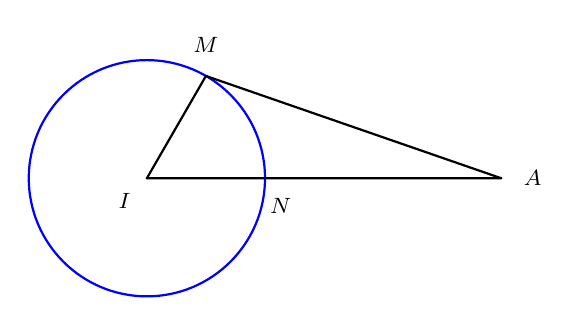
\begin{tikzpicture}[declare function={R=10;}, >=stealth, scale=0.15, line join=round, line cap=round, font=\footnotesize] 
				\coordinate (I) at (0,0);
				\coordinate (A) at (30,0);
				\coordinate (N) at (10,0);
				\coordinate (M) at (5,8.66);
				
				\draw[blue, thick] (I) circle (R);
				\draw[thick] (A)--(I)--(M)--(A); 
				
				\foreach \diem/\g in {I/-135, A/0, N/-60, M/90} 
				\filldraw (\diem) circle(1.5pt) node[shift={(\g:4mm)}]{$\diem$};
			\end{tikzpicture}
		}
		Quay lại bài toán. Cố định một điểm $A$ bất kỳ nằm trên nhánh của đồ thị hàm số $y=f(x)=x^3 - 10x + 2$ (như đề bài) và $M$ là điểm di động trên đường tròn tâm $I$ bán kính $1{,}2$. Theo kết quả phía trên, khoảng cách $MI$ ngắn nhất khi $M$ nằm giữa $I$ và $A$, khi đó khoảng cách nhỏ nhất này là $MA_{\min}=IA-IM=IA-1{,}2$.\\
		Khi $A$ di động, bài toán trở thành tìm giá trị nhỏ nhất của khoảng cách $IA-1{,}2$.\\
		Ta có $y=x^3-10x+2$, $y'=3x^2-10$ nên $y'=0 \Leftrightarrow \hoac{&x = \dfrac{\sqrt{30}}{3} \\ &x = -\dfrac{\sqrt{30}}{3}}$.\\
		Ta thấy $x=\dfrac{\sqrt{30}}{3}$ là điểm cực tiểu của hàm số $y$.\\
		Ta thấy điểm $A$ di động trên phần đồ thị của hàm số $y$ nằm bên phải của đường thẳng $x=\dfrac{\sqrt{30}}{3}$ nên $A\left(a; a^3-10a+2\right)$ với $a\ge \dfrac{\sqrt{30}}{3}$.\\ Ta có $I(0; 2)$ nên
		\[IA=\sqrt{(a-0)^2+\left(a^3-10a+2-2\right)^2}=\sqrt{a^6-20a^4+101a^2}.\]
		Khoảng cách $IA$ ngắn nhất khi và chỉ khi $h(a)=a^6-20a^4+101a^2$ nhỏ nhất trên $\left[\dfrac{\sqrt{30}}{3};+\infty\right)$. Đặt $a^2=t$, khi đó $t\ge \dfrac{10}{3}$.\\ Xét hàm số $g(t)=t^3-20t+101t$ trên $\left[\dfrac{10}{3};+\infty\right)$, khi đó $g'(t)=3t^2-40t+101$.\\
		Ta có $g'(t)=0\Leftrightarrow 3t^2-40t+101=0\Leftrightarrow \hoac{&t = \dfrac{20+\sqrt{97}}{3} \\ &t = \dfrac{20-\sqrt{97}}{3}}$.\\
		Bảng biến thiên của hàm số $g(t)$
		\begin{center}
			
\begin{tikzpicture}[scale=0.9]
				\tkzTabInit[nocadre=false, lgt=1.2, espcl=2.5, deltacl=0.65]{$t$ /1.5, $g'(t)$ /0.6, $g(t)$ /3}
				{$\frac{10}{3}$, $\frac{20-\sqrt{97}}{3}$, $\frac{20+\sqrt{97}}{3}$, $+\infty$}
				\tkzTabLine{,+, 0, -,0,+ }
				\tkzTabVar{- / $\frac{4090}{27}$, + / $151{,}51$, - / $9{,}97$, + / $+\infty$}
			\end{tikzpicture}
		\end{center}
		Dựa vào bảng biến thiên, $g(t)$ đạt giá trị nhỏ nhất tại $t=\dfrac{20+\sqrt{97}}{3}$.\\
		Vậy khoảng cách ngắn nhất giữa hai điểm nằm trên hai mô đất là
		\[IA_{\min}-1{,}2=\sqrt{g\left(\dfrac{20+\sqrt{97}}{3}\right)}-1{,}2\approx 1{,}96\mathrm{\,(m)}.\]
	}
\end{ex}
%%%=============================%%%

%%%=============EX_21=============%%%
\begin{ex}%[0D0V2-5]%[TDMT05]%[Bồ Văn Hậu]
	\immini[thm]{Cho ba chiếc hộp, hộp I đựng $8$ viên bi đỏ và $5$ viên bi xanh, hộp II và hộp III ban đầu chưa đựng viên bi nào, các viên bi có cùng kích thước và khối lượng. Tiến hành lấy ngẫu nhiên $3$ viên bi từ hộp I bỏ vào hộp III, sau đó tiến hành lấy ngẫu nhiên $4$ viên bi từ hộp I bỏ sang hộp II, sau đó lại tiếp tục tiến hành lấy ngẫu nhiên $3$ viên bi từ hộp II bỏ vào hộp III. Hãy tính xác suất để trong hộp III có đúng $4$ viên bi màu đỏ (\textit{làm tròn kết quả đến hàng phần trăm}).}{
		\begin{tikzpicture}[
			box/.style={draw=blue, thick, minimum width=3cm, minimum height=1.5cm, align=center},
			ball_red/.style={circle, fill=red, draw=black, inner sep=3pt},
			ball_blue/.style={circle, fill=cyan, draw=black, inner sep=3pt},
			ball_empty/.style={circle, fill=gray!60, dashed, inner sep=3pt},
			arrow/.style={-Stealth, thick, blue!80!black, dashed},
			scale=0.8, transform shape, font=\footnotesize]
			
			\node[box] (H1) at (0,4) {};
			\node[above] at (H1.north) {\textbf{Hộp I}};
			\foreach \x/\y in {-0.6/-0.5, 0/-0.5, 0.3/0.5, 0.9/0.5, -0.9/0, -0.3/0, 0.3/0, 0.3/-0.8}
			\node[ball_red] at ([shift={(\x,\y)}]H1.center) {};
			\foreach \x/\y in {-0.9/0.5, -0.3/0.5, 0.6/-0.5, -0.3/-0.8, 0.9/0}
			\node[ball_blue] at ([shift={(\x,\y)}]H1.center) {};
			
			\node[box] (H2) at (6,4) {};
			\node[above] at (H2.north) {\textbf{Hộp II}};
			\foreach \x/\y in {0.5/0.5, 0.5/-0.5, -0.5/0.5, -0.5/-0.5}
			\node[ball_empty] at ([shift={(\x,\y)}]H2.center) {};
			
			\node[box] (H3) at (3,0) {};
			\node[above] at (H3.north) {\textbf{Hộp III}};
			\foreach \x/\y in {0.5/-0.5, 0.5/0, 0.5/0.5, -1/-0.5, -0.5/0, -0.5/-0.5}
			\node[ball_empty] at ([shift={(\x,\y)}]H3.center) {};
			
			\draw[arrow] (H1.south) -- node[left, black, font=\small] {Lấy 3 bi} (H3.north west);
			\draw[arrow] (H1.east) -- node[above, black, font=\small] {Lấy 4 bi} (H2.west);
			\draw[arrow] (H2.south) -- node[right, black, font=\small] {Lấy 3 bi} (H3.north east);
		\end{tikzpicture}
	}
	\par
	\shortans[0]{0{,}41}
	\loigiai{
		Ta xem như có một hộp lớn IV chứa hai hộp I và II. Ban đầu ta xem hộp IV có chứa $8$ viên bi đỏ và $5$ viên bi xanh.\\
		Khi đó
		\begin{itemize}
			\item Lấy ngẫu nhiên $3$ viên bi từ hộp I bỏ vào hộp III thì ta xem như lấy ngẫu nhiên $3$ viên bi từ hộp IV bỏ vào hộp III.
			\item Lấy ngẫu nhiên $4$ viên bi từ hộp I bỏ sang hộp II thì ta xem các viên bi này vẫn nằm trong hộp IV.
			\item Lấy ngẫu nhiên $3$ viên bi từ hộp II bỏ vào hộp III thì ta xem như lấy ngẫu nhiên $3$ viên bi từ hộp IV bỏ vào hộp III.
		\end{itemize}
		Bài toán lúc này sẽ được phát biểu lại như sau: \lq\lq Hộp IV có chứa $8$ viên bi đỏ và $5$ viên bi xanh. Lấy ngẫu nhiên $6$ viên vi từ hộp IV chuyển sang hộp III. Tính xác suất để lấy được đúng $4$ viên bi màu đỏ (tức là lấy được $4$ bi đỏ và $2$ bi xanh)\rq\rq.
		\begin{itemize}
			\item Gọi $\Omega$ là không gian mẫu, suy ra $n(\Omega)=\mathrm{C}_{13}^6=1\,716$.
			\item Biến cố $A$ là \lq\lq Lấy được $4$ bi màu đỏ và $2$ bi màu xanh\rq\rq. Suy ra $n(A)=\mathrm{C}_{8}^4\cdot \mathrm{C}_{5}^2=700$.
		\end{itemize}
		Vậy xác suất $\mathrm{P}(A)=\dfrac{n(A)}{n(\Omega)}=\dfrac{700}{1\,716}=\dfrac{175}{429}\approx 0{,}41$.
	}
\end{ex}
%%%=============================%%%

%%%=============EX_22=============%%%
\begin{ex}%[TDMT05]%[Đình Nguyên]%[0D8C2-5]
		Có tất cả $18$ hình vuông nhỏ đặt cạnh nhau thành một hàng ngang. Ta tiến hành tô màu cho các hình vuông, mỗi hình vuông hoặc tô màu đỏ hoặc tô màu xanh, sao cho không có hai ô màu đỏ cạnh nhau và không có nhiều hơn hai ô màu xanh cạnh nhau. Hỏi có tất cả bao nhiêu cách tô màu cho $18$ hình vuông nhỏ này?		
		\begin{center}
			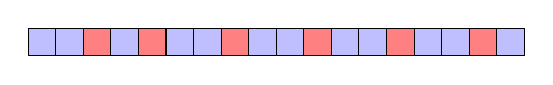
\begin{tikzpicture}[scale=0.35, font=\footnotesize, line join=round, line cap=round, >=stealth]
			\foreach \x/\y/\z in {0/blue/25, 1/blue/25, 2/red/50, 3/blue/25, 4/red/50, 5/blue/25, 6/blue/25, 7/red/50, 8/blue/25, 9/blue/25, 10/red/50, 11/blue/25, 12/blue/25, 13/red/50, 14/blue/25, 15/blue/25, 16/red/50, 17/blue/25} {
				\draw[fill=\y!\z] (\x,0) rectangle (\x+1,1);
			}
		\end{tikzpicture}
		\end{center}
		\par
		\shortans[0]{265}
	\loigiai{
		Gọi $n$ là số ô vuông cần tô màu. Gọi $T_n$ là số cách tô màu thỏa mãn điều kiện đề bài cho $n$ ô vuông.
		Ta phân loại các dãy thỏa mãn dựa trên kết thúc của chúng
		\begin{itemize}
			\item $a_n$ là số cách tô kết thúc bằng ô đỏ (... XĐ hoặc ... XXĐ).
			\item $b_n$ là số cách tô kết thúc bằng đúng một ô xanh (... ĐX).
			\item $c_n$ là số cách tô kết thúc bằng đúng hai ô xanh (... ĐXX).
		\end{itemize}
		Ta có các mối liên hệ sau
		\begin{enumerate}
			\item Để kết thúc bằng đỏ, ô trước đó phải là xanh hoặc hai ô xanh nên $a_n = b_{n-1} + c_{n-1}$.
			\item Để kết thúc bằng một ô xanh, ô trước đó phải là đỏ nên $b_n = a_{n-1}$.
			\item Để kết thúc bằng hai ô xanh, ô trước cách đó $2$ ô phải là một ô đỏ nên $c_n = a_{n-2}$.
		\end{enumerate}
		Thay vào ta có công thức truy hồi cho $a_n$ là $a_n = a_{n-2} + a_{n-3}$.\\
		Tổng số cách tô là $T_n = a_n + b_n + c_n = a_n + a_{n-1} + a_{n-2}$. Suy ra $T_n$ cũng tuân theo công thức truy hồi
		\[T_n = T_{n-2} + T_{n-3}.\]
		Thật vậy,
		\allowdisplaybreaks
		\begin{align*} 
			T_{n-2} + T_{n-3} &= (a_{n-2} + a_{n-3} + a_{n-4}) + (a_{n-3} + a_{n-4} + a_{n-5}) \\ 
			&= (a_{n-2} + a_{n-3}) + (a_{n-3} + a_{n-4}) + (a_{n-4} + a_{n-5}) \\ 
			&= a_n + a_{n-1} + a_{n-2} \\ 
			&= T_n.
		\end{align*}
		Ta xác định các giá trị cơ bản
		\begin{itemize}
			\item Với $n=1$, các cách là Đ, X nên $ T_1 = 2$.
			\item Với $n=2$, các cách là ĐX, XĐ, XX nên $ T_2 = 3$.
			\item Với $n=3$, các cách là ĐXX, ĐXĐ, XĐX, XXĐ nên $ T_3 = 4$.
		\end{itemize}
		Áp dụng công thức truy hồi để tính đến $n=18$.
		\begin{itemize}
			\item $T_4 = T_2 + T_1 = 3 + 2 = 5$.
			\item $T_5 = T_3 + T_2 = 4 + 3 = 7$.
			\item $T_6 = T_4 + T_3 = 5 + 4 = 9$.
			\item $T_7 = 7 + 5 = 12$; $T_8 = 9 + 7 = 16$; $T_9 = 12 + 9 = 21$.
			\item $T_{10} = 16 + 12 = 28$; $T_{11} = 21 + 16 = 37$; $T_{12} = 28 + 21 = 49$.
			\item $T_{13} = 37 + 28 = 65$; $T_{14} = 49 + 37 = 86$; $T_{15} = 65 + 49 = 114$.
			\item $T_{16} = 86 + 65 = 151$; $T_{17} = 114 + 86 = 200$; $T_{18} = 151 + 114 = 265$.
		\end{itemize}
		Vậy có tất cả $265$ cách tô màu.
	}
\end{ex}
%%%=============================%%%
\Closesolutionfile{ans}
\newpage
\indapan{12}{ans/ansTN-Dung}
\indapan[TF]{2}{ans/ansTN-DungSai}
\indapan[SA]{6}{ans/ansTN-DienKhuyet}
%%%%%%%%%%%%%%
%%nhãn kết thúc đề (để đếm số trang tự động mỗi đề)
\label{B\thedeso}